\graphicspath{{./}{./figures/}{./figures/synthexplore/}}

% Principle curve stuff could be neat
% \iffalse
% Other stuff to add:

% * 1d navigation
% * Principle curve: https://pypi.org/project/prinpy/ (https://web.stanford.edu/~hastie/Papers/Principal_Curves.pdf)
% \fi


\chapter{Visualizing Synthesizer Sounds}
\label{ch:visualization}
In this chapter I present Synth Explorer, a prototype of an automatic synthesizer programming interface built on top of the torchsynth synthesizer. Synth Explorer is an interactive visual browsing interface for torchsynth that was built with goal of supporting both novice and expert users in the process of navigating and developing an understanding of the vast and complex sonic space expressed by a synthesizer. It builds upon previous research in the area of sound visualization and the design is informed by concepts from the the fields of creativity support tools (CSTs) and music interaction [need cites]. These concepts, along with the taxonomy of automatic synthesizer programming interaction approaches presented in \S\ref{chapter:asp-background} grounds the the development of Synth Explorer, and provides a framework for the development of future systems. Synth Explorer is an example of an exploratory interface, with potential for inclusion of additional interactions, such as an example-based interface.

The target audience of Synth Explorer is music producers and creatives who require the use of synthesized sounds for a project. 

Kristina Andersen interviewed experienced music producers and asked them about their experience 

% During conversations with experienced music producers conducted by Kristina Andersen, participants expressed the difficulties with searching for sounds through list-based interfaces and the effort involved with organizing sound files in a way that supported their individual workflow \cite{andersen2016conversations}. Several participants expressed a desire for tools that would aid them in the process of finding sounds while promoting happy accidents. A particular emphasis was placed on the role of tools aiding in the creative process as opposed to taking over the process. The field of creative music information retrieval has also had the focus of finding ways to address the challenges of searching for sounds \cite{humphrey2013brief}. Visual browsing interfaces have been identified as beneficial for allowing users to navigate large collections of sounds more efficiently than traditional list based methods \cite{turquois2016exploring}.



It is focused on enabling users to quickly navigate both the parameter space and the perceptual space represented by a software synthesizer through an interactive visual representation of the sound.

produced by a software synthesizer through a visual representation of the sound. S

Synth Explorer is intended to support the navigation of synthesizer sounds, allowing users to develop a "sound palette" for their project which they can download and transfer into their audio workstation of choice. In addition to supporting exploration, Synth Explorer is designed with the novice user in mind. While the interface includes some technical audio terms, the drag and drop interface is modelled off of an interaction modality that will be familiar to most computer users and will allow anyone to quickly start constructing visualizations and exploring sounds. The inclusion of the technical names will allow users to begin to build up an understanding of the different dimensions of sound and how they relate to the underlying synthesizer parameters.


The design of this tool was informed by concepts put forth by research in HCI, specifically creativity support tools (CSTs) and music interaction. Based on these concepts, a framework for developing synthesizer interfaces that support creativity is presented.

\section{Introduction}
% This is pretty standard introduction material:

% The use of audio synthesizers is commonplace in creative fields including audio production, music, film, television, and games. Synthesizers are powerful and expressive devices that enable users to craft a wide range of sounds to fit the needs of their project. Because sound generation is parameterized, they offer advantages over the use of prerecorded sounds in terms of flexibility and expressiveness. However, with this flexibility comes the technical overhead required to understand how a synthesizer functions and how to adjust parameters in the correct way to achieve the desired result. The relationship between parameters and the end sonic result is typically non-linear and un-intuitive. Additionally, a typical software synthesizer might have 100+ parameters. To become proficient requires years of dedicated study and a deep understanding of sound design. The alternative is to use preset parameter settings (presets) which have been designed by experienced users. While this approach is helpful for novice users in getting started, searching through lists of named presets can be uninspiring and time consuming. Desires for improved methods for interacting with synthesizers was confirmed in a recent user study conducted by Krekovic et al. \cite{krekovic2019insights}, pointing to the need for further work in this area.

% The field of automatic synthesizer programming has been an active area of research since the late 1970s, focused on addressing the challenges associated with working with synthesizers \cite{justice1979analytic}. Despite the amount of previous work in this field, little change has been realized in commercial synthesizer interfaces. During conversations with experienced music producers, participants expressed the difficulties with searching for sounds through list-based interfaces and the effort involved with organizing sound files in a way that supported their individual workflow \cite{andersen2016conversations}. Several participants expressed a desire for tools that would aid them in the process of finding sounds while promoting happy accidents. A particular emphasis was placed on the role of tools aiding in the creative process as opposed to taking over the process. The field of creative music information retrieval has also had the focus of finding ways to address the challenges of searching for sounds \cite{humphrey2013brief}. Visual browsing interfaces have been identified as beneficial for allowing users to navigate large collections of sounds more efficiently than traditional list based methods \cite{turquois2016exploring}. 

% Maybe include some of the background from visualzations above 
In this work, Synth Explorer is proposed, an interactive visual browsing interface for synthesizer sounds with the goal of supporting both novice and expert users in the process of navigating and developing an understanding of the vast and complex sonic space expressed by a synthesizer.

Synth Explorer is a synthesizer browsing interface that builds upon previous research in the area of sound visualization and utilizes design methodology from the field of creativity support. It is focused on enabling users to quickly navigate large collections of sounds produced by a software synthesizer through a visual representation of the sound. Synth Explorer is intended to support the navigation of synthesizer sounds, allowing users to develop a "sound palette" for their project which they can download and transfer into their audio workstation of choice. In addition to supporting exploration, Synth Explorer is designed with the novice user in mind. While the interface includes some technical audio terms, the drag and drop interface is modelled off of an interaction modality that will be familiar to most computer users and will allow anyone to quickly start constructing visualizations and exploring sounds. The inclusion of the technical names will allow users to begin to build up an understanding of the different dimensions of sound and how they relate to the underlying synthesizer parameters. 

% Introduce the task of programming synthesizers -- why is it hard?
% -- structured conversations 
% -- Krekovic reference

% HCI / Creativity support background
% -- Constructing visualizations?
% -- Something on interaction?
% -- CST in music / other fields?

% Introduce Synth Explorer
% -- Prototype of a web tool to support synthesizer sound exploration
% -- Intermediary step during production, user can turn to this tool
% to create a sound palette for the music making session
% -- Provides the user with control over constructing sound layouts, specifically enables the user to choose the dimensions (spatial and color)
% -- 

\section{Background and Related Work}

% Some previously written fluff on CSTs and music interaction
% \subsection{Human Computer Interaction}
% \subsubsection{Creative Support Tools}
% Automatic synthesizer programming can be viewed from the perspective of trying to solve a human computer interaction (HCI) problem. How can a synthesizer user more effectively communicate their creative ideas to a synthesizer? Currently users are expected to learn the domain language from the perspective of whatever synthesis algorithm they are using. Can a user instead communicate their ideas to a synthesizer in a way that fits their creative needs? Creativity support is an emerging field of study that is interested in answering questions similar to this. It is focused on the development of tools that enable and enhance the creative output of an individual or group, both novices and experts. Creativity support tools (CSTs) \cite{shneiderman2007creativity} span a wide array of application domains including visual art, textiles, cooking, and music. A central question that CSTs ask is: 
% \begin{quote}
%     "How can designers of programming interfaces, interactive tools, and rich social environments enable more people to be more creative more often?"
% \end{quote}

% Too much detail - maybe put this in the last chapter
% Shneiderman \cite{shneiderman2007creativity} outlines a set of design principles for developing creativity support tools which include: support exploratory search, enable collaboration, provide rich history keeping, design with low thresholds, high ceilings, and wide walls. In subsequent related work, Davis \textit{et al.} focus on the role that CSTs play in supporting novices engaging in creative tasks and the relationship that the environment plays in creativity \cite{davis2013toward}. In their work, the authors identify two types of novice users: domain novices and tool novices. Domain novices are new to both the creative domain as well as using the creativity support tool. Tool novices have experience with the creative domain, but are novices at using a particular tool. To help evaluate and promote the development of creativity support tools for novices, they also propose a theory of creativity support based on cognitive theory.

% These concepts provide an important platform for beginning to develop tools to support users of synthesizers. Both types of novices described by Davis \textit{et al.} are common and serve to benefit from the development of improved methods for interacting with them; domain novices are both new to sound design / music production as well as to using a specific synthesizer, whereas a tool novices would likely have experience with sound design / music production, but would be a novice with using a specific synthesizer.

% This is also a bit too in detail
% \subsubsection{Music Interaction}
% Music and Human-Computer Interaction \cite{holland2013music}, or Music Interaction. Research related to the use of interactive systems that involve computes for any kind of musical activity. Music interaction draws heavily from other areas of HCI research, but also responds to the needs and desires of the music community. There are unique considerations in the context of musical applications that makes music interaction different from other fields of HCI. A musical instrument is not a utilitarian tool whose development should be ever-improved to make it more efficient. Musical instruments are played, and sometimes that is the only goal. Tomaka [cite me!] identifies that imperfections and limitations of a musical instrument give an instrument character. McDermott \cite{mcdermott2013should} identifies the importance of engagement in musical interaction and the relation that bears to the concept of \textit{flow} \cite{csikszentmihalyi1990flow}. The learning curve plays is crucial to the level of engagement that a player experiences when playing a musical instrument, both in the short-term and long-term. Holland \cite{holland2013music} concludes, "In order to remain engaging, consuming and flow-like, activities that involve musical instruments must offer continued challenges at appropriate levels of difficulty: not too difficult, and not too easy."

\subsection{Creativity Support}
% Copying to the background:
The field of creativity support is focused on the development of tools to enable and enhance the creative output of both novice and expert users. Creativity support tools (CSTs) span a wide array of application domains including visual art, textiles, cooking, and music. Davis \textit{et al.} focus on the role that CSTs play in supporting novices engaging in creative tasks and the relationship that the environment plays in creativity \cite{davis2013toward}. 
% This was discussed in the background chapter
In their work, the authors identify two types of novice users: domain novices and tool novices. Domain novices are new to both the creative domain as well as using the creativity support tool. Tool novices have experience with the creative domain, but are novices at using a particular tool. To help evaluate and promote the development of creativity support tools for novices, they also propose a theory of creativity support based on three cognitive theories: embodied creativity, situated creativity, and distributed creativity.

Embodied creativity is based on the premise that creativity is intrinsically linked to the interaction that a user has with their environment. It is through interacting with their world that an individual is able to make creative ideas more concrete and express themselves.

Situated creativity is related to the concept of flow. In the context of creativity support, situated creativity is linked to how much effort a user must apply when using a tool to carry out a task. As a user becomes more comfortable with a tool, it gradually starts to feel like a natural extension of their body and they are enabled to explore deeper expression of their creativity.

Distributed creativity is focused on the tasks that a human can offload to a particular tool during a creative task. By handing over a portion of a creative task to a support tool, a novice user may be able to arrive at rewarding results earlier in the process, thereby motivating them to continue to engage in the creative process and enhance their skills.

Using these theories as a guide, Andrews proposed a novel 2D interface for exploring and generating graphics \cite{10.1145/3325480.3325506}. Their work used an algorithmic method for generating 2D graphics, which a user is able to interact with to control the generation of new graphics. Because of the vastness of the space of potential images that could be generated by the algorithm, the user interface utilizes a spatial layout of images to allow the user to quickly assess a set of possibilities which they can then use to guide the generation of further images. While this interface was focused on the generation of images, the interaction ideology is similar to that of Synth Explorer, which is built on top of an algorithmic audio synthesis engine; the space of possible sounds that a synthesizer can produce is far too vast for a user to navigate all at once, so a small random subset of that space is initially presented and the user is then able add more sounds and hone in on a particular result.

The following subsections present several examples of creativity support tools specific to the process of exploring large collections of sounds as well as working with synthesizers.

\subsection{Creative Music Information Retrieval}
% The field of music information retrieval (MIR) is a growing research area that was born out of the need to navigate increasingly large collections of digital music. Creative MIR is a subset of the field that is focused on applying the techniques from MIR towards creative applications including music production \cite{humphrey2013brief}. 

Visualization of sounds based on sound similarity has been studied in depth and is reviewed by Cooper \textit{et al.} \cite{cooper2006visualization}. Work that is particularly relevant to Synth Explorer is DrumSpace, a 2D visualization interface developed by Turqois \textit{et al.} for exploring large collections of drum sounds \cite{turquois2016exploring}. A component of their study was a subjective evaluation that compared user experiences in browsing for drum sounds using a traditional list-based layout of samples to 2D visual layouts. For the 2D layouts they compared one method that automatically sorted sounds based on sound similarity against one that organized sounds based on the filename. Users reported having a significant preference for for the 2D based layout, but had no significant preference for the type of layout. Participants were able to explore a much larger number of audio examples in a shorter period of time when using the 2D interfaces. Turqois \textit{et al.} also identified that the layout based on sound similarity caused some confusion to the users; the layout was based on a set of audio features which had been reduced to 2D using a dimensionality reduction technique called t-SNE \cite{van2008visualizing}, because algorithms like t-SNE create complex combinations of higher dimensional features into a lower dimensional embedding for visualization, the meaning of the resulting dimensions used for visualization are often hard to identify. Turqois \textit{ et al.} also suggest that color could be a helpful addition to the interface. Building upon this work, Shier \textit{et al.} conducted further experiments on the perceptual relevance of different methods of dimensionality reduction techniques for visualizing drum samples in 2D and identified MDS as having the highest correlation with user similarity ranking \cite{shier2021manifold}.Synth Explorer builds on these tools and leverages similar techniques for creating 2D visualizations of synthesizer sounds.

\subsection{Automatic Synthesizer Programming}
The field of automatic synthesizer programming is focused on the development of algorithmic methods for creating synthesizer parameter settings and has been an active area of research since the late 1970s \cite{justice1979analytic}. Since then, a large body of work has emerged incorporating contemporary work from machine learning. One of the major tasks that has been studied is known as sound matching, or inverse synthesizer \cite{yee2018automatic}. During inverse synthesis a user provides a target sound as input to an algorithm and receives an estimate for parameter settings for a synthesizer to reproduce the target sound as accurately as possible. The development of novel user interfaces has also been a focus in automatic synthesizer programming including the use of vocal imitations \cite{cartwright2014synthassist}, interactive algorithms based on genetic programming \cite{yee2016use}, macro controls \cite{esling2019universal}, and semantic descriptors \cite{seago2013new}. Synth Explorer is inspired by the same driving motivation behind these works, which is to provide a more intuitive approach to programming synthesizers. Synth Explorer is related to the data-driven approach used by in SynthAssist \cite{cartwright2014synthassist}; all the sounds used in Synth Explorer are pre-computed and audio features are stored in a database which is queried.

\section{Design}
Synth Explorer is designed to support exploration and provide a low threshold of entry for users to begin working with synthesized sounds within a creative context. The tool is aimed at tool novices \cite{davis2013toward}: users who may have expertise in composing music and working with digital audio workstations, however have limited experience in working with audio synthesizers. Synth Explorer is expected to be an accessory tool used during the creative process of composing digital music in addition to a users' main digital audio workstation. For example, a user might be composing a film soundtrack in their workstation of choice and find that they are desiring to add a new synthesized instrument to their score. In this example, the user would open up Synth Explorer, browse for a sound that fits their needs, and then load those sounds back into their workstation. While navigating between two different programs may seem like an impediment to the creative flow, it is hypothesized that the added benefits of the Synth Explorer interface will outweigh the inconvenience of switching between programs.

The user interaction methodology was designed according to the theories of cognition presented by Davis \textit{et al.} for supporting novice users working with CSTs: embodied creativity, situated creativity, and distributed creativity \cite{davis2013toward}. The design of Synth Explorer in relation to these three aspects is presented below.

\subsubsection{Embodied Creativity}
The browsing interface should support embodied creativity -- the layout and interaction with the browsing interface should utilize multiple modes of sensory cognition to facilitate understanding. Spatialization of multimedia objects based on similarity has been used in previous related work \cite{10.1145/3325480.3325506} and is used here to provide deeper insight into the relationship between sounds. Based on the previous issues identified with 2D visualizations of sound which caused confusion to users \cite{turquois2016exploring}, the user here is given control over how the visualization is constructed to empower them to develop an understanding of the spatial relationship between sounds. Specifically, users are able to assign audio features to the x, y, and color of each sound object on the 2D layout.

\subsubsection{Situated Creativity}
Synth Explorer should support a user in maintaining creative flow whilst working on their project. Additionally, the user interface should have a low threshold of entry to enable novices to quickly start engaging with sounds and working towards realizing their creative goal. The conscious effort required to use Synth Explorer should quickly dissipate into the subconscious, allowing the user to instead focus the entirety of their attention on the creative task at hand.

% Maybe this should go above in introduction.
%X \textit{et al.} identified that music producers often feel like the task of browsing for sounds using traditional methods is tedious and takes them out of the creative flow. Similarly, X \textit{et al.} identified that synthesizer users felt like programming sounds in software synthesizer interfaces was complex and required time and effort. Users' in their study expressed

\subsubsection{Distributed Creativity}
Synth Explorer should offload the laborious task of organizing large collections of sounds and navigating the sonic space represented by a particular synthesizer. The system should also not take full control over the creative process and provide the end user with room to express creative control. In a traditional synthesizer a user would either need to learn how to program sounds themselves, rely on experts to create and organize presets, or organize presets themselves. Applying distributed creativity to Synth Explorer, the user should offload the task of programming and organizing synth presets over to the system and shift their energy to the task of curating a selection of sounds that fit the needs of their creative vision.

\section{Implementation}
\subsection{Sound Generation and 2D Mapping}
The core of Synth Explorer is the synthesizer. For this work a python based modular synthesizer called \textit{torchsynth}\footnote{\url{https://github.com/turian/torchsynth}} is being used. \textit{torchsynth} is a versatile synthesis engine designed for fast audio generation. A set of synthesizer presets was automatically generated by randomly sampling the parameter space of  \textit{torchsynth}, four second long audio files for the patches saved, and a set of audio features computed on those audio files.

Audio features are designed to capture perceptually relevant aspects of audio in a compact format. In DrumSpace, the 2D visualization of samples was produced by computing a set of audio features and then performing dimensionality reduction to two-dimensions using t-SNE \cite{turquois2016exploring, van2008visualizing}. In subsequent work, the UMAP dimensionality reduction algorithm \cite{mcinnes2020umap} was found to be an effective alternative to t-SNE in terms of time-complexity and visualization quality \cite{jiale2020visualization}. Synth Explorer uses two different UMAP embeddings as options for visualization: an embedding based on mel-frequency cepstral coefficients, and an embedding based on spectral features \cite{peeters2004large}. In addition to these dimensionality reduced embeddings, a set of eight low-level audio features computed using librosa\footnote{\url{https://librosa.org/doc/latest/index.html}} are included. The keyboard pitch is also included in the set of available features that can be used for constructing a visualization.

The database of audio files and associated features allows the synthesizer sound space to be automatically organized based on these various features. This addresses the distributed creativity component of the design. The user offloads the task of generating synthesizer sounds and organizing them to the system. Due to the speed of the synthesis system and audio feature extraction process, nearly ten thousand unique sounds can be generated and analyzed in about 20 minutes. This corresponds to over ten hours of synthesized audio. Listening to and organizing all these sounds would be impractical, or at least mundane, for any user, novice or expert. 

Instead of forcing a layout on the end user, the user has the ability to decide which feature / embedding they want to use to construct their visualization. This decision was made based on participant feedback that they were confused by the sound similarity visualization used in DrumSpace \cite{turquois2016exploring}. An attempt is made to address this issue by explicitly providing the user with a set of features ranging from concrete (keyboard pitch) to more abstract (spectral embedding using UMAP), and allowing them to decide which they want to use to create the visualization. Additionally, tooltips are provided for each feature which provides an opportunity for the user to learn more about the underlying dimensions and their relationship to audio perception.

\subsection{Browsing Interface}
Using the guiding cognitive theories for developing creativity support tools, an interface was designed based on the aforementioned related work. A drag and drop interface, an interaction paradigm common to consumer computer user interfaces, is employed, allowing users to assign different features to the dimensions of the visualization. The final interface is shown in figure \ref{fig:ui_1}. % include piece on embodied creativity and situated creativity
The workflow of the interface is divided into four different sections: adding sounds, constructing the visualization, exploring and saving sounds, and downloading saved sounds. An overview of each step in the workflow is provided in the following sections.
\begin{figure*}
    \centering
    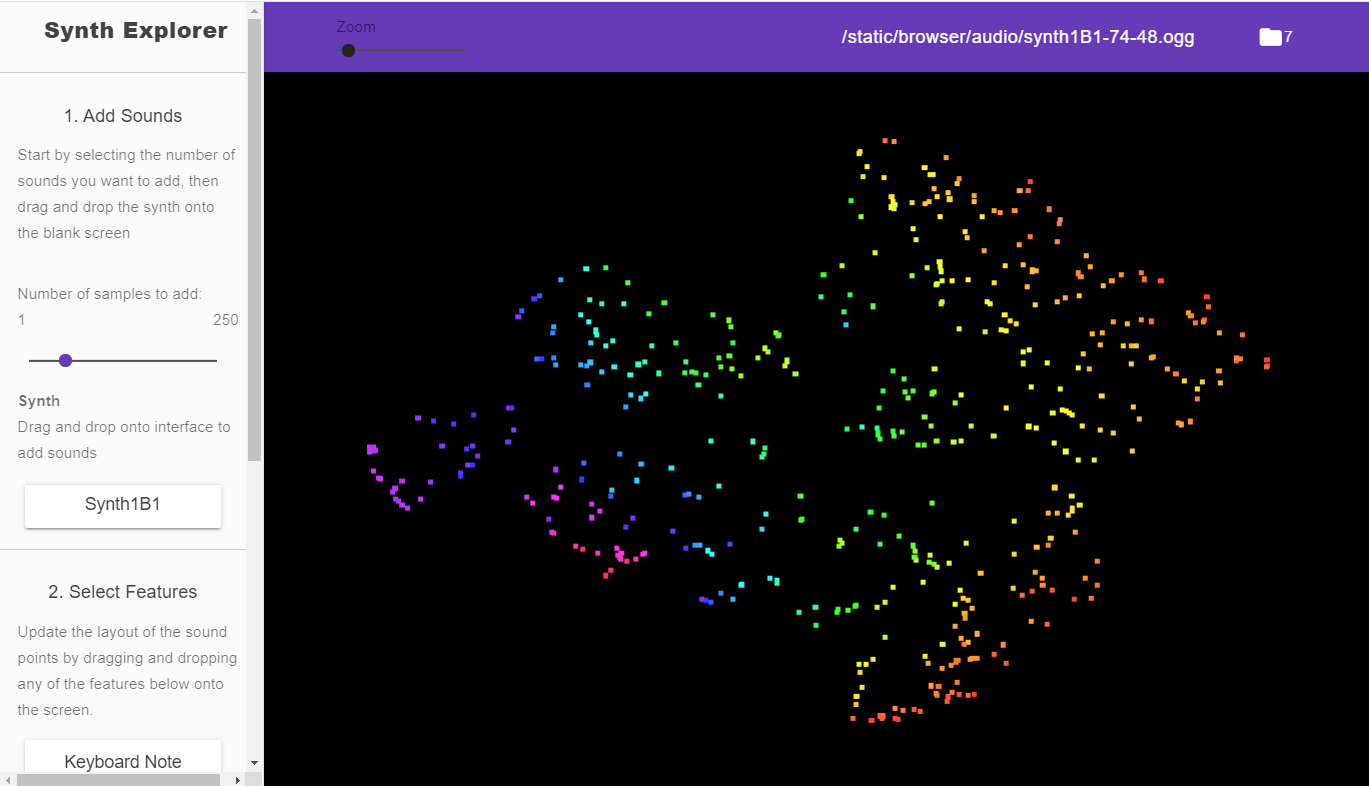
\includegraphics[width=0.9\textwidth]{SynthExplore Init.png}
    \caption{Synth Explorer User Interface}
    \label{fig:ui_1}
\end{figure*}

\subsubsection{Adding Sounds}
It was mentioned earlier that the space of possible sounds that can be produced by a synthesizer is vast. The example of producing ten thousand four second audio clips of patches from \textit{torchsynth} represents only a subset of the possible sounds the synthesizer is capable of producing. Presenting a user with ten thousand audio clips on a 2D layout would also be overwhelming. The user is initially presented with a small random subset of possible outcomes. The user is given the option to control how many sounds are added to the visualization at once using a slider control that ranges between 1 and 250. They are then able to add that many sounds to the their visualization by dragging and dropping the UI object representing a particular synthesizer onto the visualization area. This section of the user interface is shown in figure \ref{fig:steup 1}. Currently only one synthesizer is shown in the interface, however any number could be included. This would allow the user to compare and explore multiple synthesizers at any given time. 

Once a user drops a synthesizer onto the visualization, the requested number of synthesizer sounds are randomly selected from the database and added to the interface. A single sound is represented as a single point on the 2D visualization.

\begin{figure}
    \centering
    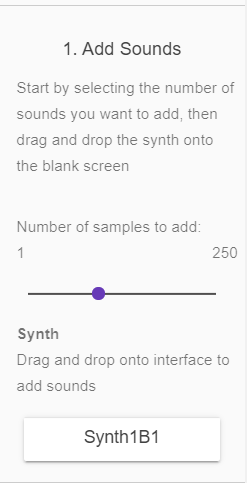
\includegraphics[width=0.3\linewidth]{SynthExplore_AddSounds.png}
    \caption{Synth Explorer Step 1}
    \label{fig:steup 1}
\end{figure}

\subsubsection{Constructing the visualization}
The next section of the user interface is focused on allowing the user to control their visualization. Specifically, this section allows users to decide which features are assigned to which dimension of the visualization. The available features are shown on the left side of user interface in figure \ref{fig:features}. Using the same drag and drop paradigm, the user is able to drag any of the features onto the visualization surface in order to modify the layout of audio samples. When the user initiates a drag and drop interaction, large drop areas representing the different dimensions of the visualization appear for the user to choose from. The available dimensions are the x-axis, y-axis, and the color of the points. Once a feature is dropped onto one of the dimensions of the visualization, the points representing the sounds automatically shift into the new position to reflect the changes. Any feature can be associated with any dimension, allowing the user to explore the relationship between the features and develop a visualization that meets their needs.

A decision was made to use the technical names of the features. While this may be confusing to some users, there are unfortunately not many great alternatives to this problem. Tooltips are provided to give novices an approximate non-technical description of the feature -- the hope is that these users will still feel inspired to explore these different features and learn their effect on the resulting visualization.

\begin{figure*}
    \centering
    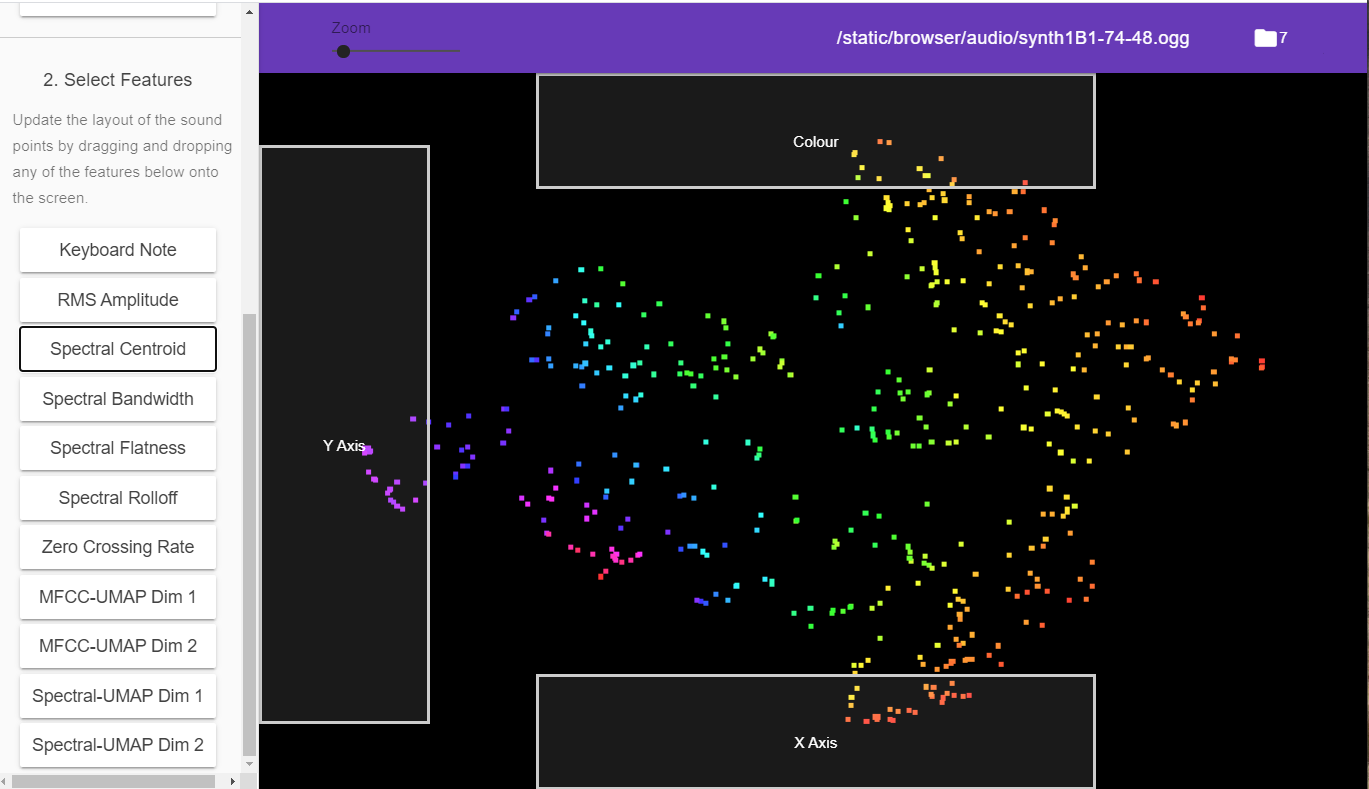
\includegraphics[width=0.9\textwidth]{SynthExplore A.png}
    \caption{Synth Explorer UI: Updating features}
    \label{fig:features}
\end{figure*}


\subsubsection{Exploring and Saving Sounds}
The majority of the space on the user interface is occupied by the 2D browsing space, which is shown in figure 2. This is the space where synthesizer sounds are represented as points on a scatter plot. To listen to a particular sound, the user simply needs to hover their curser over the point representing a sound. They receive both auditory and visual feedback once they intersect with a point. The sound represented by the point plays and a small circle burst the same color as the point is animated into view at the point of interaction. Users can also zoom into the visualization using their mouse scroll wheel and navigate the space using a click and drag operation. Each of these gestures is meant to reflect operations that would feel intuitive and natural to an experienced computer user.

This mode of interaction provides a fast way for the user to preview a large number of samples. The goal of the 2D layout and exploration method is to provide the user with an embodied method for exploring sounds. The 2D spatial layout using colors provides users with a visual representation of the sonic space that they can interact with and create their own associations with. The interaction itself is easy to master as it simply requires dragging a mouse around the screen and listening to sounds. Modifying the layout using drag and drop interactions also requires little conscious effort. These intuitive interactions were implemented to support situated creativity and thereby aid creative flow.

When a user has listened to a sound that they like and want to save, they can press the 's' key on their keyboard to save that clip to a 'sound palette'. This is equivalent to adding an item to an online shopping cart. The user can then continue to explore sounds.

At this point the user is able repeat any of the preceding steps and continue explore the visualization: add more sounds, modify the dimensions with different features, explore the space, and save sounds.

\subsubsection{Downloading}
Once the user has sufficiently explored the sonic space and saved a palette of sounds they would like to use, they can click on the download icon next to their saved sounds and download all the synthesizer sound files they saved. Once they have done this they are free to use those sounds for whatever creative task they would like.

\subsection{Technical Implementation Details}
Synth Explorer is implemented as a web application. The Django framework\footnote{\url{https://www.djangoproject.com/}} was used to implement the backend of the web app. Django is written in python and provides an elegant data-model system for interacting with a database such as MySQL\footnote{{https://www.mysql.com/}}. The sound generation and analysis portion of the application is written as a Django management command -- when this command is run, a set of sounds is rendered using \textit{torchsynth}, and analyzed using librosa and UMAP. Once the samples have been analyzed and audio files saved to disk, the audio features and patch settings for each sound is saved in a MySQL database.

The frontend of the application is written using HTML, CSS, and JavaScript. The foundation of the application was based on code developed by Leon Feddden \footnote{\url{https://github.com/fedden/umap_tsne_embedding_visualiser}}. This code was modified to function within the Django framework and the user interaction paradigm was modified to support dynamic adding of synthesizer samples and user construction of the layout using drag and drop interactions. The visualization and animation is rendered using three.js\footnote{\url{https://threejs.org/}}.


\section{Evaluation}
\subsection{Creativity Support Index}
Synth Explorer was evaluated using the creativity support index (CSI) questionnaire based on two separate tasks:

\textbf{Task 1: Synthesizer browsing for an existing project}

In this task the user is working on an existing musical project in a separate workstation. They are composing a piece of music and then are asked to find a new synthesizer sound for an additional track to their composition. They must leave the workstation,
open Synth Explorer, browse for a new sound, then leave Synth Explorer and open the new sound back in the workstation they were initially working within.

\textbf{Task 2: Creating a sound palette for a new project}

In this task the user is beginning a new project and is searching for a set of synthesizer sounds to create the sonic palette for the new composition. They may have a particular sound in mind, but are asked to explore the interface in an open-minded way to look for new sounds and create a collection as inspiration to start the new project.

\subsection{CSI Results}
Results of the CSI evaluation are shown in table \ref{table:csi}. These results show that Synth Explorer supported task 1 to a greater degree than task 2. Task 1 received an overall score of 78.67 whereas task 2 received an overall score of 71.67. The results showed that collaboration was not supported and received a score of zero for both tasks. This makes sense considering the nature of the tasks and the tool itself. Collaboration was not a part of the evaluated tasks, however, the tool itself does not currently support collaboration in any meaningful way other than allowing two users to sit next to each other and browse for synth sounds simultaneously. The tool supported exploration in both tasks more than any of the other attributes evaluated. This result is positive considering that was one of the major goals for the tool. Another area that was well supported by the tool is enjoyment, while the results and expressiveness of the tool itself were not highly rated. The lack of expressiveness also makes sense for the tool; Synth Explorer itself does not necessarily allow expression -- it allows a user to explore sounds with the goal of maintaining a creative flow in a large creative context, but it is more challenging to actually be expressive with the tool.

The results section of the evaluation did not score highly either. This was due to the fact that the 2D layout of sounds was still challenging to navigate and make sense of. This is in part due to the underlying method for generating sounds as well as the sound mapping techniques. Randomly sampling a synthesizer is not the best way to capture meaningful sounds from the synthesizer and a lot of times produces dramatic or unusable results. This lead to a large portion of the sounds being a bit too wild for the tasks at hand. Additionally, capturing sound similarity in two dimensions is still an open question that requires further work. Despite this, the interface was effective at enabling rapid exploration of a large number of sounds and it was enjoyable getting to explore manipulating the visualization by dragging and dropping the different features onto the plot.

\begin{table}[th]
\centering
\begin{tabular}{l|llll|ll}
Area           & Q1 & Q2 & T1 & T2 & T1 Total   & T2 Total \\
\hline
Collaboration  & 1  & 1  & 0            & 0            & 0              & 0            \\
Enjoyment      & 7  & 8  & 5            & 4            & 75             & 60           \\
Exploration    & 10 & 7  & 5            & 5            & 85             & 85           \\
Expressiveness & 5  & 4  & 1            & 2            & 9              & 18           \\
Immersion      & 8  & 7  & 3            & 2            & 45             & 30           \\
Results        & 5  & 6  & 2            & 2            & 22             & 22           \\
Total Score    &    &    &              &              & \textbf{78.67} & \textbf{71.67} 
\end{tabular}
\caption{Results of creativity support index questionnaire.}
\label{table:csi}
\end{table}

\section{Discussion}
Overall I am really pleased with the results of this project. I have spent quite a bit of time working with synthesizers and visualizing audio using techniques from MIR, however was missing a more structured approach to designing the user interface that works on top of these systems. Situating the development of this tool in the context of creativity support theory felt like a natural extension of the work and I think has lead to a much more engaging and useful final result. That being said, there is still a lot of room for improvement in this design. The CSI evaluation exposed a couple important weaknesses in the system that can be addressed in future iterations on this project.

I was surprised by the results of the CSI evaluation as well -- intuitively I felt like the second task would be better supported by the tool based on my experience using the tool, however the numerical results showed a different result. This is interesting and caused me to reflect on the evaluation and the design of Synth Explorer. This pointed out on aspect of the system where the second task performed more highly, expressiveness, however resulted in an overall lower score due to the lower results from the questions relating to expressiveness. This makes sense in context of the system and adding more opportunities for increased creativity and expressiveness within the interface would be an interesting area to explore.

\section{Future Work and Conclusion}
This paper has introduced the Synth Explorer creativity support tool. The intention of this tool is to support users in the process of working with synthesizers and finding new sounds for creative projects. A further goal of the tool is to support novice users who might have experience in music production, but do not have experience working with synthesizers. Synth Explorer was designed to support novices using an approach to creativity support based on cognitive theory which emphasizes embodied, situated, and distributed creativity. The designed tool uses a 2D visualization of synthesizer sounds to arrange sounds spatially as well as uses colors to support an embodied approach to exploration. By using a simple drag and drop interface and quick browsing of sounds using a visual layout, users are able to quickly start exploring and remain engage in their creative task.

An evaluation of the tool using the creativity support index revealed insight into the strengths and weaknesses of the tool and helped to identify some areas for potential further work. The most glaring limitation of the tool is it's lack of support for collaboration. The current version of the system has no support for collaboration, however this could be added relatively easily based on the implementation. Since Synth Explorer is built as a web application using the Django framework, a user login system could be added quite easily which would allow users to save and share collections of sounds that they have curated. Different synthesizers and layouts could also be shared through a system like this. Another limitation of the current system is in the available options to filter and search for sounds. Currently the user is limited to added random samples to the interface and exploring different configurations of that. In order to support users in arriving at more useful results and collections of sounds, providing additional search options such as a search by similarity or providing additional tools for selecting and filtering the current selection would be a good area for future work as well.